\documentclass[9pt]{report}

\usepackage{talks}
\newcommand{\expect}[1]{\mathbb{E}\!\left[ #1 \right]}
\newcommand{\reals}{\mathbb{R}}
\newcommand{\draw}[2]{#1^{(#2)}}
\usepackage{mathpazo}
\usepackage{sourcecodepro}

\begin{document}


\sf%
\mbox{ }
\\[12pt]
\spc{{\LARGE\bfseries \color{MidnightBlue}{Orders of Magnitude:}}}
\\[8pt]
\spc{\Large\bfseries \color{MidnightBlue}{Stan Algorithms and Engineering}}
\\[36pt]
\noindent 
\spc{\large\bfseries \color{MidnightBlue}{Bob Carpenter}}
\\[2pt]
\spc{\small Center for Computational Mathematics}
\\[2pt]
\spc{\small Flatiron Institute}
\vfill 
\noindent 
\spc{\footnotesize June 2023}
\hfill

\includegraphics[width=1.5in]{img/flatiron_logo.png}

\includegraphics[width=0.5in]{img/stan-logo.png}

\sld{Flatiron Institute}
\begin{quote}
The \myemph{mission} of the \myemph{Flatiron Institute} is to
\myemph{advance scientific research} through
\myemph{computational methods}, including data analysis, theory, modeling and simulation.
\end{quote}
\begin{itemize}
\item \myemph{Center for Computationa}: Math (stats/ML), Biology, Neuroscience, Astrophysics,
  Quantum Physics
\item part of \myemph{Simons Foundation}
  \begin{subitemize}
  \item US\$300M+ science and education grants per year
  \item US\$5B endowment
    \end{subitemize}
\end{itemize}

\sld{Pop Quiz}
\begin{itemize}
\item Who's the \myemph{most famous Stan} in \myemph{St.\ Louis}?
\end{itemize}

\sld{Stan the Man \hfill (active 1941--1963)}
\begin{itemize}
\item Not Ulam. Not a stalker fan.
\item \myemph{Stan ``The Man'' Musial}.  Outfielder, \myemph{\slshape St. Louis Cardinals.}
\end{itemize}
\begin{center}
  \spc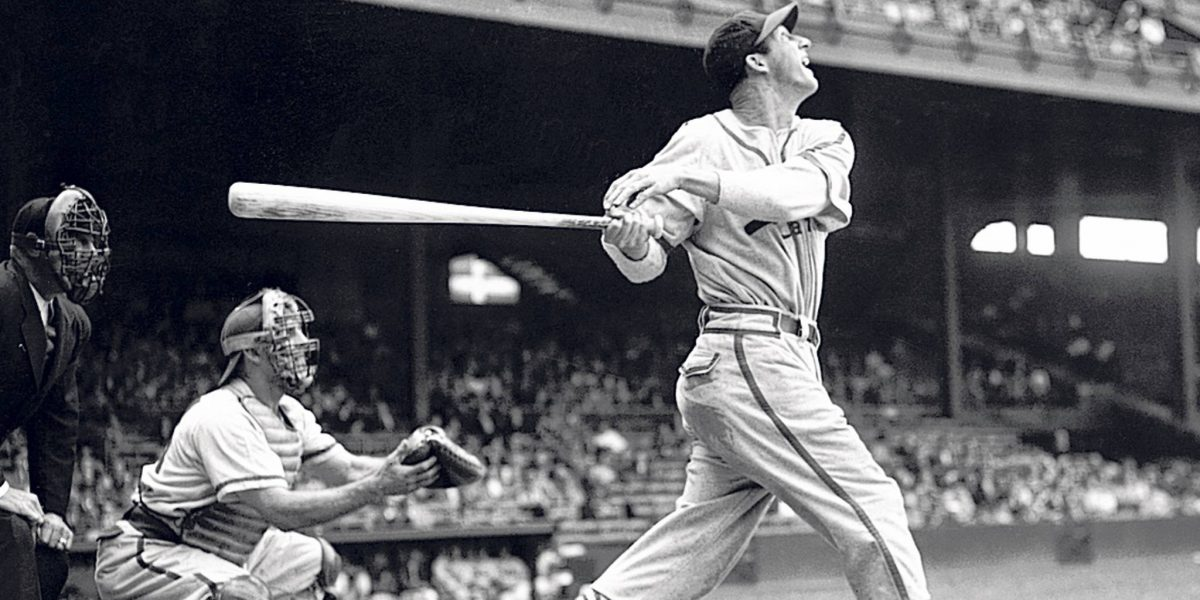
\includegraphics[width=0.6\textwidth]{img/stan-the-man.jpeg}
  \\
  {\small {\slshape Wikipedia}: One of the \myemph{greatest and most consistent} hitters in baseball}
  \end{center}


  \sld{}
  \vspace*{-24pt}
\begin{center}
    \spc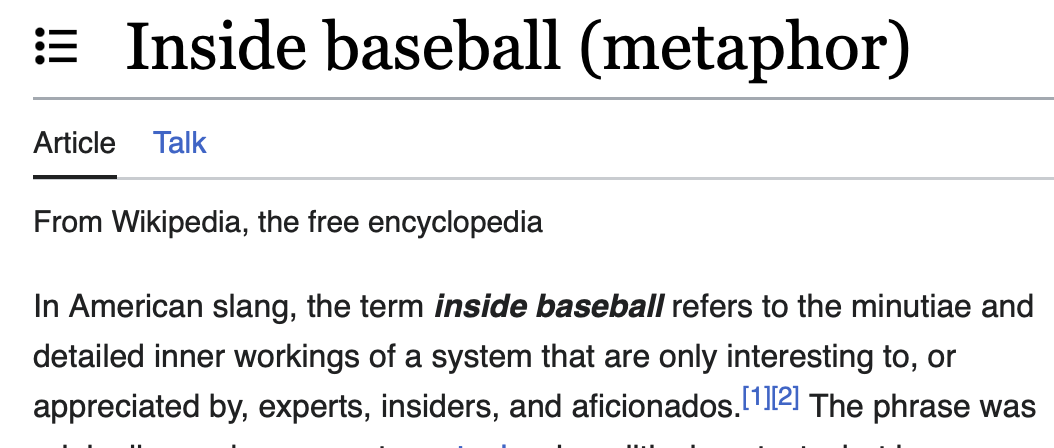
\includegraphics[width=\textwidth]{img/inside-baseball.png}
  \end{center}
  \vfill
  \null

  
\sld{Swing for the fences}
\begin{itemize}
\item 2011: I move \myemph{from industry to Columbia} to work with 
  Gelman. 
\item I was \myemph{getting scooped} on crowdsourcing. 
\item Michael Collins (CS) suggests I \myemph{work on harder problems}.
\item I \myemph{listened} and we started the \myemph{Stan} project.
\end{itemize}
\begin{center}
  \spc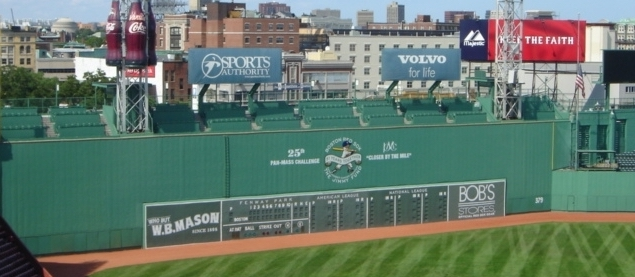
\includegraphics[width=0.6\textwidth]{img/fenway-fences.jpeg}
\end{center}


  
\sld{Where are the fences?}
\begin{itemize}
  \item \myemph{Sometimes}: an \myemph{unknown unknown}.
  \item \myemph{Usually}: about an \myemph{order of magnitude} away
  \item I'm a \myemph{computer scientist}, so that's only \myemph{$
      \mathbf{\times\, 2}$}  \hfill   ($\approx$\ Gelman \& Hill) 
  \end{itemize}
\vfill
\begin{center}
  \spc
  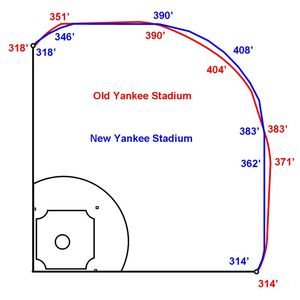
\includegraphics[height=1in]{img/yankee-stadium.jpeg}
  \hfill
  \spc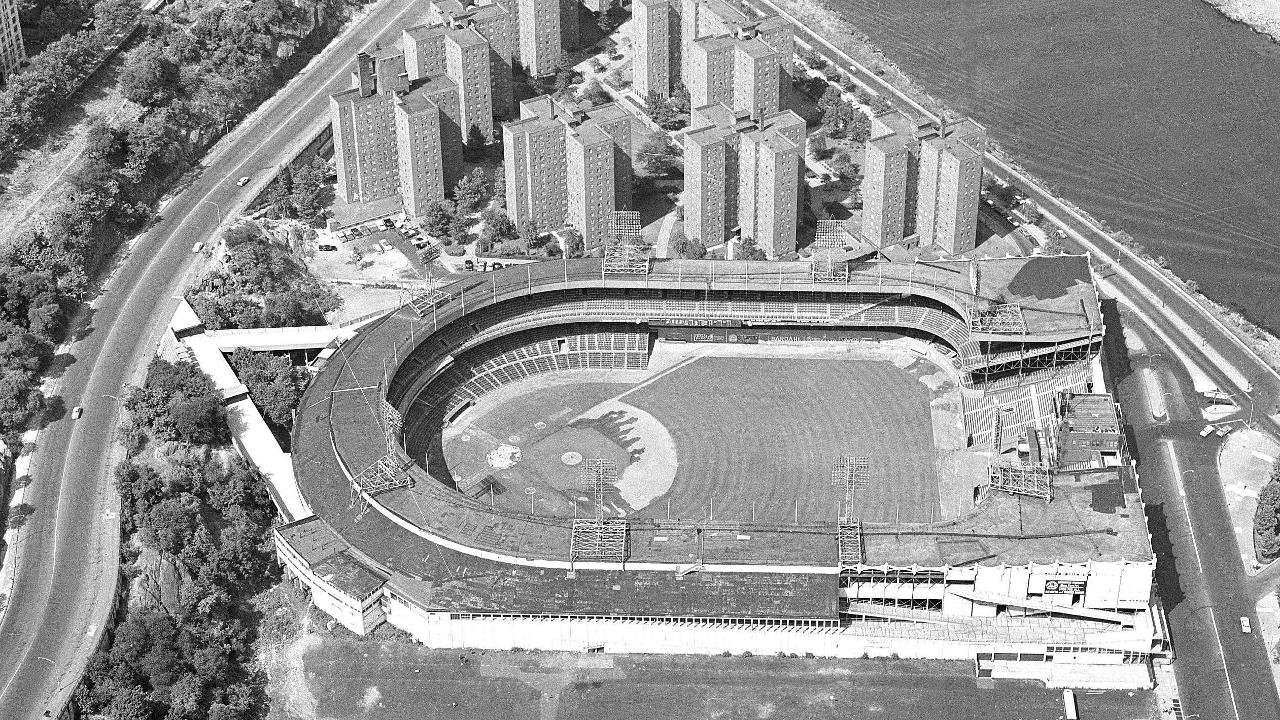
\includegraphics[height=1in]{img/polo-grounds.jpeg}
  \hfill
  \spc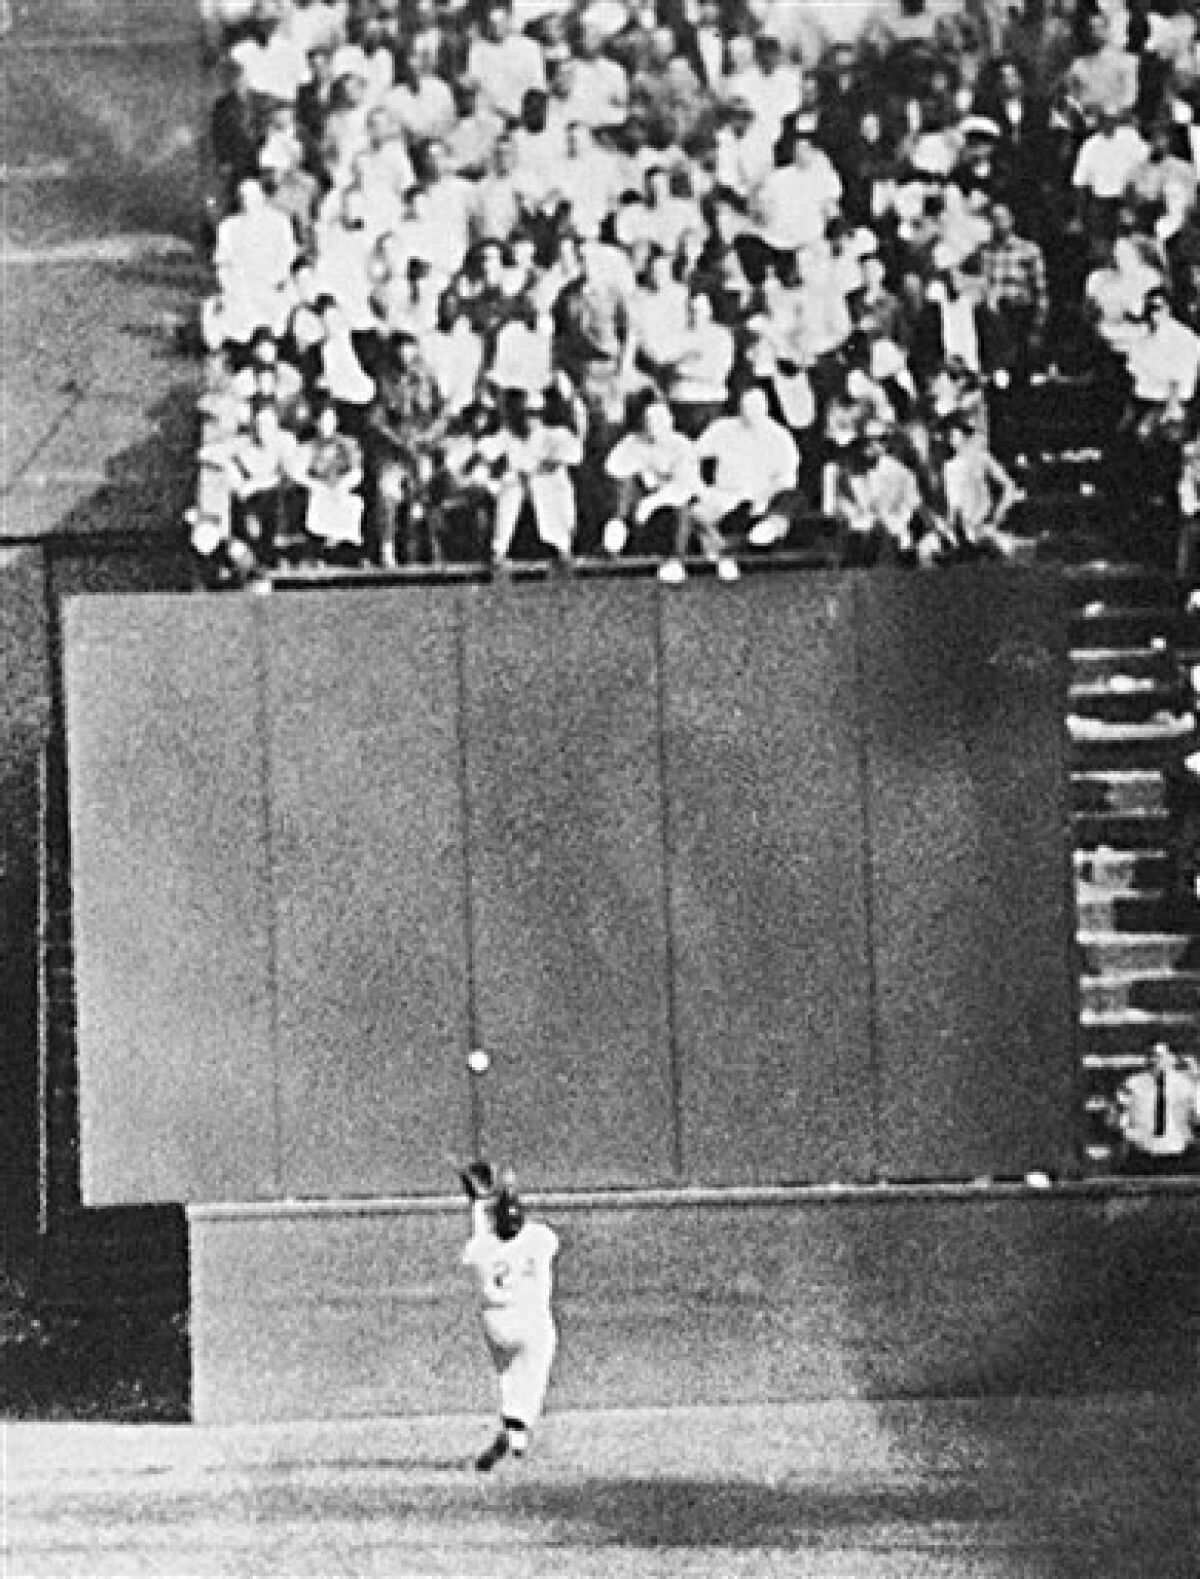
\includegraphics[height=1in]{img/willie-mays.jpeg}
\end{center}

\sld{}
\vfill 
\begin{center}
\Huge \myemph{Part I\\[12pt] MCMC for Bayes}
\end{center}
\vfill 
\vfill 

\sld{Bayesian Inference \hfill\normalsize (Bayes $\approx$ 1750,
  Laplace $\approx$ 1800)}
\begin{itemize}
\item \myemph{unknown} (parameters) $\theta \in \reals^D;$ \quad 
  \myemph{observed} (data) $y \in \reals^N$
\item \myemph{Estimation}: 
$$
\widehat{\theta}
= \expect{\theta \mid y}
= \int_{\reals^D} \theta \cdot p(\theta \mid y) \, \textrm{d}\theta. 
$$
\item \myemph{Event probabilities}
$$
\Pr[A \mid y]
= \expect{\textrm{I}_{A}(\theta) \mid y}
= \int_{\reals^D} \textrm{I}_{A}(\theta) \cdot p(\theta \mid y) \, \textrm{d}\theta. 
$$
\item \myemph{Posterior prediction}
$$
p(\tilde{y} \mid y) 
= \expect{p(\tilde y \mid \theta) \mid y}
= \int_{\mathbb{R}^D} p(\tilde{y} \mid \theta) \cdot p(\theta \mid 
  y) \, \textrm{d}\theta. 
$$
\end{itemize}

\sld{Monte Carlo \hfill {\normalsize (Fermi, von Neumann, Ulam
    $\approx$ 1930s--1940s)}}
\begin{itemize}
\item Go-to approach to \myemph{high-dimensional integration}
\item \myemph{Randomized algorithm} for deterministic integrals 
$$
\expect{f(\theta)] \mid y}
\approx \frac{1}{M} \sum_{m = 1}^M f\!\left(\draw{\theta}{m}\right) 
$$
for \myemph{independent and identically distributed} (i.i.d.) draws 
$$
\draw{\theta}{m} \sim p(\theta \mid y) 
$$
\item Proof: \myemph{central limit theorem} (CLT)
  + law of \myemph{unconscious statistician}. 
\end{itemize}

\sld{Markov chain Monte Carlo \hfill \normalsize(Ulam, late 1940s)}
\begin{itemize}
\item When \myemph{too hard to draw i.i.d.}\ from posterior.
\item Draw $\draw{\theta}{0}, \ldots, \draw{\theta}{M}$ from a
  homogeneous \myemph{Markov chain}
\begin{align}
\draw{\theta}{0} &\sim q_0(\theta)
  \\[8pt]
  \theta_{m + 1} &\sim q(\theta_{m + 1} \mid \theta_{m}).
\end{align}
\item \myemph{Ergodic theorem} says we can use MCMC just like MC, when chain
  \begin{subitemize}
  \item is \myemph{irreducible} (doesn't get stuck),
  \item is \myemph{aperiodic} (doesn't visit partition cyclically), and
  \item has \myemph{stationary distribution} s.t.\
    $\draw{\theta}{m + 1} \sim p(\theta \mid y)$ if
    $\draw{\theta}{m} \sim p(\theta \mid y).$
  \end{subitemize}
\item Proof: equilibrium convergence + law of unconscious statistician
\end{itemize}

\sld{Accept/reject balance \hfill \normalsize(Metropolis et al.\ 1950)}
\begin{itemize}
\item \myemph{propose} $\theta^* \sim q(\theta \mid \theta_{m})$,  
  \begin{subitemize}
  \item where $q$ is \myemph{symmetric}, i.e.,  $q(\theta' \mid \theta) = q(\theta \mid \theta')$
  \end{subitemize}
  \item \myemph{accept} with probability  
$\displaystyle  
\min\!\left( 1,  \
  \frac{p(\theta^* \mid y)}
       {p(\theta_m \mid y)}
     \right)$
\renewcommand{\baselinestretch}{1.2}
{\small\bfseries
\begin{verbatim} 
theta[0] = q0_rng()
for m in range(M):
   theta_star = q_rng(theta[m])
   u = uniform_rng(0, 1)
   accept = log(u) < log p(theta_star) - log p(theta[m])
   theta[m + 1] = theta_star if accept else theta[m]
\end{verbatim}
}
\renewcommand{\baselinestretch}{1.0}
\end{itemize}

\sld{Non-reversible proposals \hfill \normalsize (Hastings 1970)}
\begin{itemize}
\item \myemph{propose} $\theta^* \sim q(\theta \mid \theta_{m})$, 
  \begin{subitemize}
  \item where $q$ is \myemph{not necessarily symmetric}
  \end{subitemize}
  \item \myemph{accept} with probability 
$\displaystyle 
\min\!\left( 1, 
  \frac{p(\theta^* \mid y)}{p(\theta_m \mid y)}
    \cdot 
    \frac{q(\theta_m \mid \theta^*)}{q(\theta^* \mid \theta_m)}
     \right)t$
\item If $q$ is symmetric, second term drops out, reduces to Metropolis
\end{itemize}

\sld{Detailed Balance}
\begin{itemize}
\item Let $p(\theta_{m + 1} \mid \theta_m)$ be the Markov chain
  \myemph{transition kernel}
  \begin{subitemize}
  \item reject probability makes it mixed discrete/continuous
  \end{subitemize}
\item Metropolis-Hastings \myemph{accept} step ensures MCMC kernel satisfies
  \myemph{detailed balance},
  $$
  p(\theta \mid y) \cdot p(\theta' \mid \theta)
  = p(\theta' \mid y) \cdot p(\theta \mid \theta').
  $$
  \vspace*{-12pt}
  \begin{subitemize}
    \item ensures chain has stationary distribution $p(\theta \mid y)$
    \item given irreducibility and aperiodicity
      \end{subitemize}
\end{itemize}

\sld{HMC \hfill \normalsize(Duane et al.\ 1987)}
\begin{itemize}
\item \myemph{couples momentum} $\rho \in \mathbb{R}^D$ to sample over
  \myemph{phase space} $\reals^D \times \reals^D$
\item \myemph{Hamiltonian} $H(\theta, \rho) = - \log p(\theta, \rho) =
  - \log p(\theta) - \log p(\rho),$
  \begin{subitemize}
  \item \myemph{Kinetic energy}: $-\log p(\rho) = -\log \textrm{normal}(0, \textrm{I}_D) =
    \frac{1}{2}
    \cdot \theta^{\top} \cdot \theta.$
  \item \myemph{Potential energy}: $-\log p(\theta) = - \log p(\theta \mid y)$
  \end{subitemize}
\item \myemph{Hamiltonian Monte Carlo} (HMC) couples two stationary-preserving transition kernels:
  \begin{subitemize}
  \item \myemph{Exact momentum} refresh: $\rho_{m + 1} \sim \textrm{normal}(0, 1).$
  \item \myemph{Metropolis proposal}: $(\theta^*,
    -\rho^*)$, where $(\theta^*, \rho^*)$ solves Hamiltonian dynamics from initial
    $(\theta_m, \rho_{m + 1})$ to proposal $(\theta^*, \rho^*)$ at
    time $t$.
  \item Metropolis \myemph{corrects numerical integration error} solving ODE
  \item Momentum \myemph{flip for reversibility} (required, but erased)
  \end{subitemize}
\end{itemize}

\sld{Why is HMC so good?}
\begin{itemize}
\item \myemph{Long distance} proposals with \myemph{high acceptance} rates
\item \myemph{Effective sample size} (and hence \myemph{mixing}) is proportional to expected squared
  jump distance
\item An \myemph{exact solution} preserves initial Hamiltonian, so 100\% accept 
\item The \myemph{leapfrog integrator} used to solve dynamics is \myemph{symplectic}
  \begin{subitemize}
    \item steps preserve volume (hence no Hastings correction for Jacobian)
    \item symplectic integrators very good at \myemph{preserving Hamiltonian}
    \item not so great at \myemph{solving dynamics}, but doesn't matter---we
      only need \myemph{long jumps with high acceptance}
  \end{subitemize}
\end{itemize}

\sld{HMC is hard to tune}
\begin{itemize}
\item \myemph{$y$-axis}: ESS; \qquad \myemph{$x$-axis}:  step size; \qquad
  \myemph{facets}: steps
\item \myemph{blue}: $Y$; \qquad \myemph{red}: $Y^2$
\item \myemph{dashed lines}: NUTS
\end{itemize}
\begin{center}
  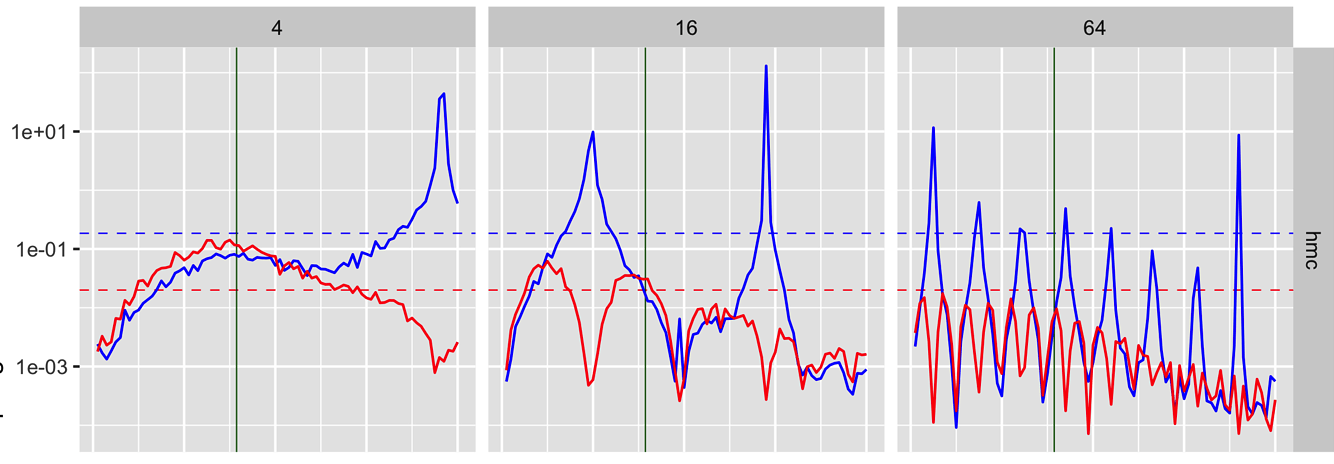
\includegraphics[width=0.9\textwidth]{img/hmc-jitter.png}
\end{center}  

\sld{HMC + Euclidean metric}
\begin{itemize}
\item add symmetric, positive-definite \myemph{metric} $M$ to
  define distance
  \begin{align}
    ||\theta|| &= \theta^{\top} \cdot M \cdot \theta
    \\[8pt]
  d(\theta, \theta') &= ||\theta - \theta'||
  \end{align}
\item Stan estimates $M$ as inverse posterior covariance,
  $$
  \widehat{M} \approx \textrm{cov}[\theta \mid y].
  $$
\item \myemph{kinetic energy} now $-\log p(\rho) = \frac{1}{2} \cdot \rho^{\top} \cdot M \cdot \rho,$
\item so \myemph{momentum refresh} $\rho \sim \textrm{normal}(0, M^{-1}).$
\end{itemize}


\sld{No-U-turn sampler (NUTS) \hfill \normalsize (Hoffman and Gelman 2013)}
\begin{itemize}
\item \myemph{Tuning HMC} dynamics (step size, number of steps) is
  \myemph{very hard}
\item No-U-turn sampler (NUTS) automatically tunes
  \begin{subitemize}
  \item \myemph{stepsize} during warmup iterations
  \item \myemph{metric} during warmup iterations
  \item \myemph{number of steps} dynamically
  \end{subitemize}
\item Betancourt (2017) added several improvements to NUTS for Stan
\end{itemize}

\sld{NUTS (cont.)}
\begin{itemize}
\item Sampling algorithm
  \begin{subitemize}
  \item randomly simulate \myemph{forward vs.\ backward} time, \myemph{doubling steps}
  \item \myemph{until U-turn} (momentum brings ends closer)
  \item \myemph{select a step} along path, \myemph{biased} toward \myemph{last
        doubling}
    \item \myemph{slice sampling}, revised to more efficient \myemph{multinomial}
    \end{subitemize}
    \begin{center}
      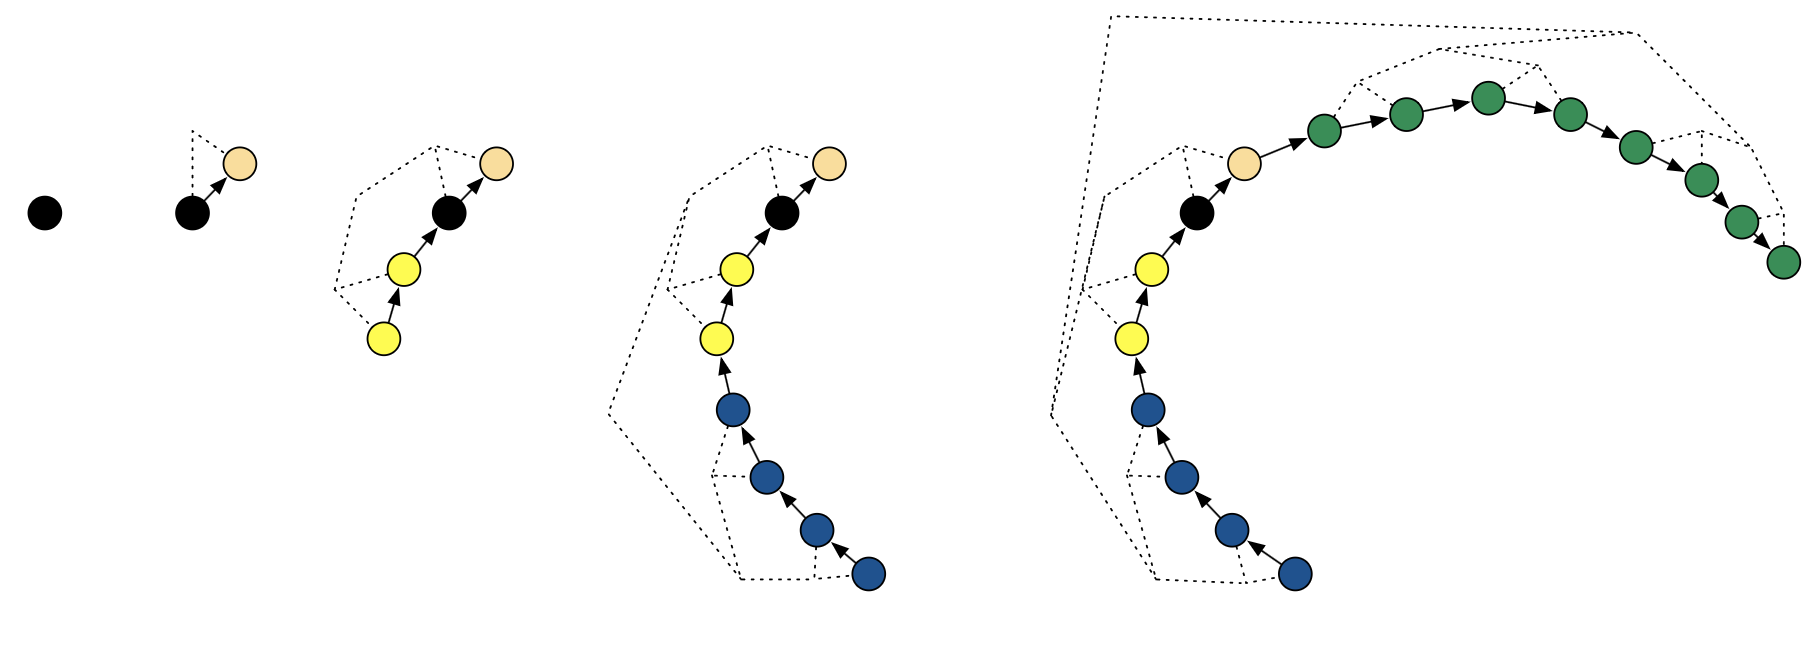
\includegraphics[width=0.725\textwidth]{img/nuts-doubling.png}
    \end{center}
  \end{itemize}

\sld{Generalized HMC \hfill \normalsize (Horowitz 1991)}
\begin{itemize}
\item Uses \myemph{partial momentum refresh}
  \begin{subitemize}
    \item preserves momentum for directed movement across posterior
    \end{subitemize}
\item Fix $\lambda \in (0, 1)$ (lower preserves more momentum)
\item \myemph{G-HMC refresh}:
  $$
  \rho_{m + 1} = \sqrt{\lambda} \cdot z_m + \sqrt{1 - \lambda}
  \cdot \rho_m,
  $$
where $z_m \sim \textrm{normal}(0, M^{-1}).$
\item This is also an \myemph{exact update}
  \begin{subitemize}
    \item i.e., if $\rho_m \sim  \textrm{normal}(0, M^{-1}),$ then $\rho_{m + 1} \sim 
    \textrm{normal}(0, M^{-1}).$
    \end{subitemize}
\end{itemize}

\sld{Uh oh!  What about the Flip?}
\begin{itemize}
\item \myemph{Why not} use G-HMC with a single step and tune $\lambda$?
\item Remember that \myemph{momentum flip}?
  \begin{subitemize}
  \item it's required for \myemph{reversibility} of Metropolis
  \item \myemph{thrown away} in basic HMC by composing momentum update
  \item but \myemph{preserved} in G-HMC
  \end{subitemize}
\item \myemph{Without high acceptance}, momentum flip produces \myemph{random walk}. 
\item High acceptance means \myemph{small step size} in Hamiltonian dynamics.
\end{itemize}

\sld{Non-reversible accept \hfill \normalsize(Neal 2020)}
\begin{itemize}
\item Instead of uniform $u$, use \myemph{sawtooth} pattern, \myemph{jittered} for ergodicity
  \begin{subitemize}
  \item \myemph{not reversible}, but \myemph{preserves stationary}
  \end{subitemize}
\item Iteration vs.\ accept probability $u$ (red reject) \myemph{groups acceptance}:
\begin{center}
  \spc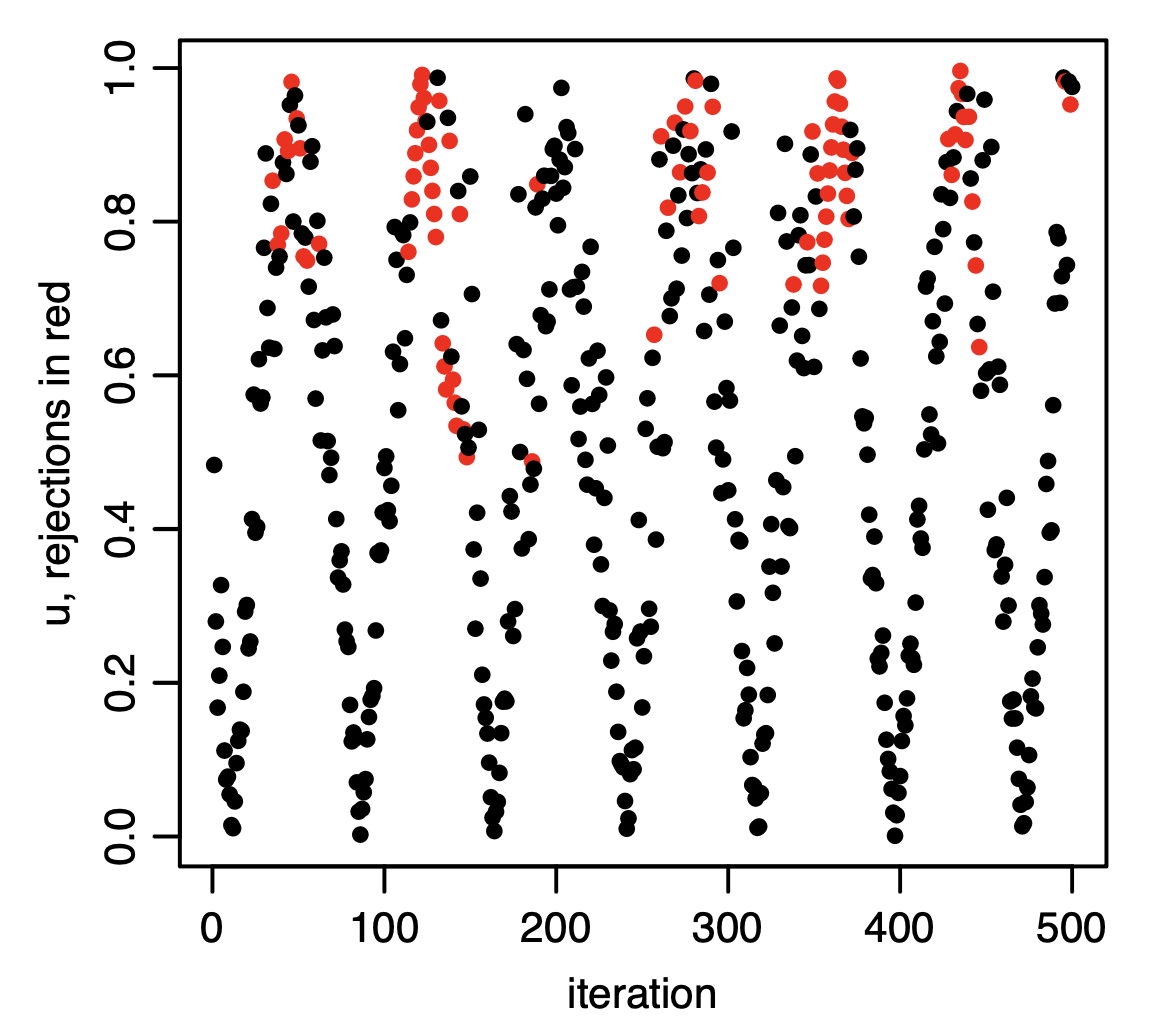
\includegraphics[height=1.5in]{img/neal-nonrevu.png}
\end{center}
\end{itemize}

\sld{Delayed Rejection \hfill \normalsize(Mira 2001)}
\begin{itemize}
\item $K$-step delayed rejection involves $K$ distinct proposals
  \begin{subitemize}
\item Step 1.  Propose and accept/reject as usual with Metropolis.
\item Step 2.  \myemph{If rejected, propose again} with a new proposal
  and accept/reject with \myemph{Metropolis-Hastings}
\\
\qquad \qquad    $\vdots$
\item Step $K$.  If rejected, propose one last time.
\end{subitemize}
\item Need \myemph{Hastings correction} to ensure detailed balance.
\item Proposals may depend on previous proposal(s).
\item \myemph{Innovation:} Only retry if acceptance probability was low 
\end{itemize}

\sld{Delayed Rejection HMC \hfill \normalsize(Modi et al.\ 2022)}
\begin{itemize}
\item \myemph{Multiple scales} (varying curvature) 
  along an \myemph{entire path}
\item Each \myemph{retry cuts step size} by constant $c$ and \myemph{multiplies steps}
  by $c$ (e.g., $c = 2$ or $c = 5$)
  \begin{subitemize}
  \item earlier attempts kept step size and extended path
  \item ours better if gradient-based \myemph{Hamiltonian diverged}
  \end{subitemize}
\begin{center}
  \spc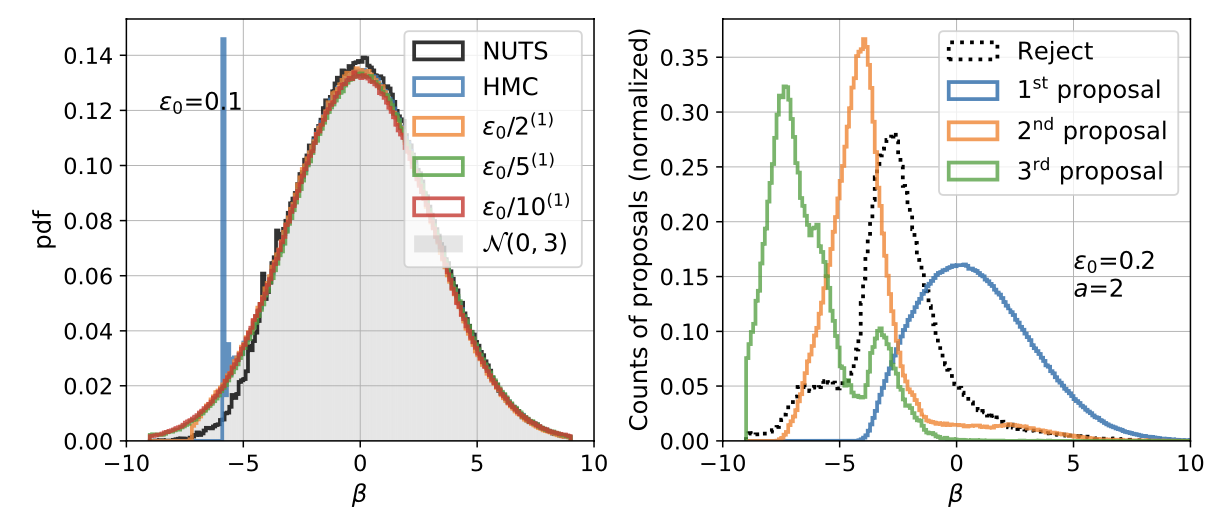
\includegraphics[height=1.1in]{img/dr.png} \ \small (funnel draws/accept)
\end{center}
\end{itemize}

\sld{MEADS \hfill \normalsize(Hoffman and Sountsov 2022)}
\begin{itemize}
\item \myemph{Massively parallel} version of Neal's non-reversible
  accept \myemph{G-HMC}
\item Uses \myemph{complementary chains for adaptation}
  \begin{subitemize}
  \item novel, efficient \myemph{principal eigenvalue} estimation of
    step size
  \item covariance in complementary chains used to \myemph{estimate metric}
  \item \myemph{accelerates adaptation}, robust to single chains
    getting stuck (Bales 2019)
  \item much easier to \myemph{parallelize}
  \item \myemph{little waste} and \myemph{easy restart}
  \end{subitemize}
\item conveniently a Markov chain \myemph{w.o.\ warmup phase}
  \begin{subitemize}
  \item still need \myemph{burn-in}
  \end{subitemize}
\end{itemize}

\sld{DR-G-HMC \hfill \normalsize(Modi, Roualdes, $\ldots$ in progress)}
\begin{itemize}
\item Apply \myemph{delayed rejection} to \myemph{generalized HMC}
\item \myemph{Retries} use \myemph{one step} instead of constant time
\item \myemph{Multiple scales} adapted \myemph{within a trajectory}
\item solves \myemph{non-centered funnel} (like DR-HMC)
\item Use MEADS-like \myemph{parallel tuning}
\end{itemize}

\sld{Convergence: nested $\widehat{R}$ \hfill
  \normalsize(Margossian et al. 2022)}
\begin{itemize}
\item \myemph{GPUs} run \myemph{1000+} parallel chains
\item \myemph{One draw}/chain \myemph{minizes wall time}
\item \myemph{Nest blocks} with \myemph{same init}; monitor \myemph{transient bias} + \myemph{variance}
\end{itemize}
\begin{center}
  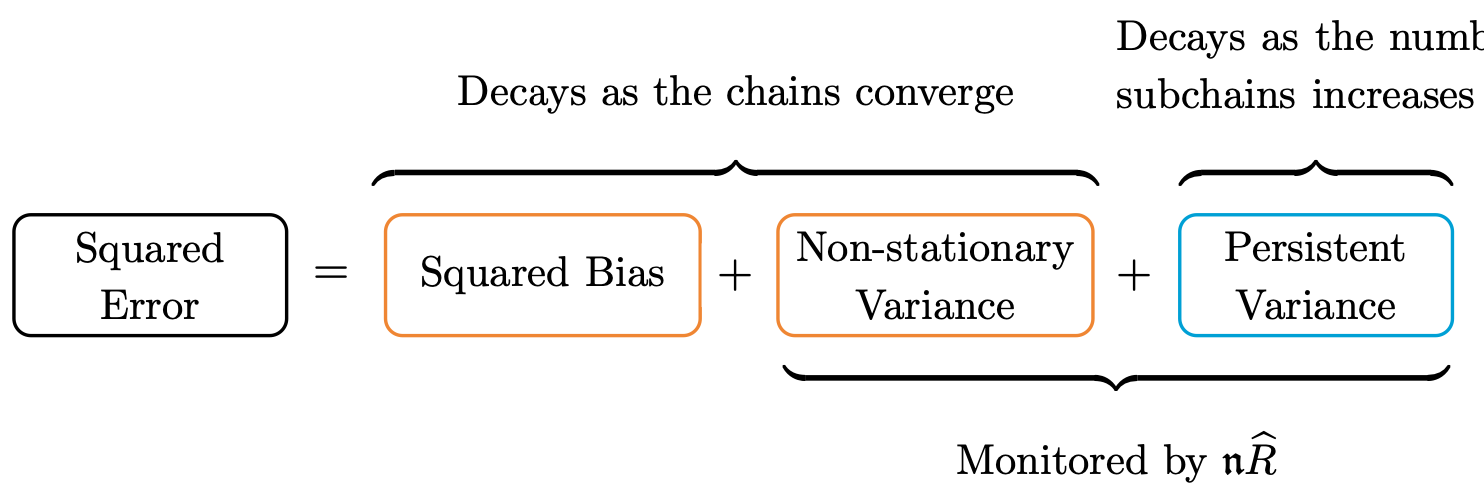
\includegraphics[width=0.9\textwidth]{img/nRhat.png}
\end{center}



\sld{}
\vfill 
\begin{center}
  {\Huge \myemph{Part II\\[12pt] Stan Language}}
\end{center}
\vfill 
\vfill 

\sld{Tuples \hfill (next release)}
\begin{itemize}
\item Required \myemph{design doc} choices
  \begin{subitemize}
  \item mainly on syntax and including \myemph{named structs}
  \end{subitemize}
\item \myemph{Massive refactoring} required in transpiler \& I/O
  (thanks Brian and Steve)
  \begin{subitemize}
    \item \myemph{my bad} in original code assuming \myemph{dense rectangular}
    \end{subitemize}
\begin{verbatim}
tuple(int, real) x = (42, 3.14);  // type & construct

int a = x.1;    real b = x.2;     // rvalue (access)

x.1 += 1;       x.2 = sqrt(x.2);  // lvalue (assign)
\end{verbatim}
\end{itemize}

\sld{Closures and lambdas \hfill (design accepted)}
\begin{itemize}
\item \myemph{Closures bind} non-local variables in function bodies
\item \myemph{Lambdas} for anonymous inline function definitions
  (C++-like syntax)
\item Full \myemph{type} support in the object language 
  \begin{subitemize}
    \item variables with function types and assignment 
    \item function arguments with function types (i.e., higher-order 
      functions) 
    \end{subitemize}
  \item Support \myemph{comprehensions} with \myemph{partial
      evaluation}
    \begin{subitemize}
    \item e.g., scalable GP kernels
      \end{subitemize}
\end{itemize}

\sld{Ragged arrays \hfill (design pending)}
\begin{itemize}
\item Not much more to say about this
\item Challenging to \myemph{statically size}
\item Need to \myemph{generalize math} library
\vfill
\item \myemph{Bigger challenge: sparse matrices}
  \begin{subitemize}
  \item Eigen C++ support is poor
  \item Have to roll our own algorithms (e.g., log determinant)
  \end{subitemize}
\end{itemize}

\sld{More types and constraints}
\begin{itemize}
\item \myemph{Orthonormal matrices} (generalizes unit vector)
  \begin{subitemize}
  \item e.g., hyperspherical statistics and rotations
  \item tricky $SO(N)$ geometry (rotation vs.\ reflection)
  \end{subitemize}
\item \myemph{Composable} transforms
  \begin{subitemize}
  \item e.g., affine compositions for hierarchical rates or probabilities
  \end{subitemize}
\item \myemph{Pluggable} transforms
  \begin{subitemize}
  \item e.g., specialized simplex transforms for scale
  \end{subitemize}
\end{itemize}

\sld{}
\vfill 
\begin{center}
  {\Huge \myemph{Part III\\[18pt] Automatic\\[12pt] Differentiation}}
\end{center}
\vfill 
\vfill

\sld{Mat-var to Var-mat \hfill\normalsize(underway)}
\begin{itemize}
\item \myemph{Reverse-mode} autodiff uses \myemph{autodiff variables}
  \begin{subitemize}
  \item one per value evaluated in the constraints and log density
  \item C++ class instance store a \myemph{value} and \myemph{adjoint}
  \item virtual function to apply chain rule 
  \end{subitemize}
\item Stan matrices currently store a \myemph{matrix of variables}
\item Moving to more efficient \myemph{variable of matrixes}
  \begin{subitemize}
  \item more \myemph{memory locality}
  \item less \myemph{copying}
  \end{subitemize}
\item \myemph{huge refactor} of math lib and transpiler
\end{itemize}

\sld{Expression templates \hfill\normalsize(well underway)}
\begin{itemize}
\item original Stan \myemph{evaluated} expression templates 
\item goal: \myemph{lazy evaluation} plus \myemph{static compilation}
\item improved Stan tries to \myemph{propagate} expression templates
  \begin{subitemize}
  \item \myemph{reduces copying}
  \item accelerate \myemph{composed code compilation}avoids eager, unnecessary copies 
  \item Fortrain-like speed; how C++ is faster than C
  \end{subitemize}
  \item very \myemph{tricky C++}
\end{itemize}

\sld{GPU kernel \hfill\normalsize(starting)}
\begin{itemize}
\item Very \myemph{expensive to move} data between GPU and CPU
\item now use where order of computation $/gg$ order of data
  \begin{subitemize}
  \item e.g., matrix-matrix multiply, Cholesky factorization,
    \myemph{not} matrix-vector multiply, dot prducts, etc.
  \end{subitemize}
\item Write \myemph{GPU code} for entire \myemph{math library}
\item \myemph{Order of magnitude (or two!)} speedup (cf. JAX)
\item \myemph{Enormous} undertaking 
\end{itemize}

\sld{}
\vfill 
\begin{center}
  {\Huge \myemph{Part IV\\[12pt] Approximate Inference}}
\end{center}
\vfill 
\vfill 
\begin{center}
{\Large  (cf. \myemph{MCMC}, which is asymptotically \myemph{exact})}
\end{center}

\sld{Laplace Approximation \hfill (released)}
\begin{itemize}
\item Given a \myemph{posterior mode}
  $$\theta^* = \textrm{arg max}_\theta \ p(\theta \mid y)$$
\item \myemph{Second-order Taylor expansion} is called \myemph{Laplace
    approximation}
  $$\theta \sim \textrm{multi\_normal}(\theta^*, (-H)^{-1}(\theta^*)),$$
  where $(-H)^{-1}$ is the inverse negative Hessian
\item pairs with our built-in gradient-based \myemph{quasi-Newton
    optimization}
  \begin{subitemize}
  \item uses \myemph{L-BFGS} for local curvature adjustment (i.e., \myemph{precondition})
  \end{subitemize}
  \vfill
\end{itemize}

\sld{Autodiff Variational Inference (ADVI)}
\begin{itemize}
\item Given posterior $p(\theta \mid y)$ on the
  \myemph{unconstrained scale}
  \begin{subitemize}
  \item i.e., $p(\theta \mid y) > 0$ for all $\theta \in \mathbb{R}^D$
  \end{subitemize}
\item \myemph{Variational approximation} is $\textrm{multi\_normal}\!\left(\theta \mid
  \widehat{\mu}, \widehat{\Sigma}\right),$ where
    $$
  \widehat{\mu}, \widehat{\Sigma}
  = \textrm{argmin}_{\mu, \Sigma}
  \ \textrm{KL}\!\left[\textrm{multi\_normal}(\theta \mid \mu, \Sigma) 
    \,\big|\big|\, p(\theta \mid y) \right]
  $$
\item \myemph{Sample} $\draw{\theta}{1}, \ldots \draw{\theta}{M} \sim \textrm{multi\_normal}\!\left(\theta \mid
    \widehat{\mu}, \widehat{\Sigma}\right),$
\item \myemph{Inverse transform} draws back to constrained scale
\item \myemph{Impovements} by (1) Welandawe, Andersen, Vehtari, and 
  Huggins (2022); (2) Domke and Agrawal (2022).
\end{itemize}

\sld{ADVI objective evaluation}
\begin{itemize}
\item KL-divergence is integral, w.\ $q(\theta) =
  \textrm{multi\_normal}(\mu, \Sigma).$
\begin{align}
  \ \textrm{KL}\!\left[\, q \ || \ p \, \right]
   &= \underbrace{\int_{\mathbb{R}^D}
     q(\theta) \cdot \log q(\theta) 
     \, \textrm{d}\theta}_{\textrm{entropy of } q}
     - \underbrace{\int_{\mathbb{R}^D}
     q(\theta) \cdot \log p(\theta \mid y)}_{\textrm{cross entropy } q
     \textrm{ to } p}
     \, \textrm{d}\theta
  \\[8pt]
   &\approx -\textrm{H}[\textrm{multi\_normal}(\mu, \Sigma)]
     + \frac{1}{M} \sum_{m = 1}^M \log p(\draw{\theta}{m} \mid y),
\end{align}
where $\draw{\theta}{m} \sim \textrm{multi\_normal}(\mu, \Sigma).$
\end{itemize}

\sld{ADVI SGD}
\begin{itemize}
\item Need \myemph{gradient} $\nabla_{\theta} \, \textrm{KL}\!\left[\,
    q \
    || \ p\,\right]$ to minimize
  $$
  \textrm{arg min}_{\mu, \Sigma} \
  \textrm{KL}\!\left[ \, \textrm{multi\_normal}(\theta \mid \mu, \Sigma) \
    \big|\big| \ p(\theta \mid y) \, \right]
  $$
\item \myemph{Entropy} term can be handled analytically or by Monte Carlo
\item \myemph{Cross-entropy} requires \myemph{stochastic gradient},
  $$
  \nabla_\theta \sum_{m = 1}^M \log p(\draw{\theta}{m} \mid y)
  =
  \sum_{m = 1}^M \nabla_\theta \log p(\draw{\theta}{m} \mid y),
  $$
  with nested derivative by \myemph{automatic differentiation}
\end{itemize}

\sld{ADVI improvements \hfill (in progress)}
\begin{itemize}
\item Need to select a \myemph{step size} \hfill
  \begin{subitemize}
  \item current algorithm too weak; parallel grid search way better
  \end{subitemize}
\item Need to select an \myemph{SGD algorithm}
  \begin{subitemize}
  \item ADVI is vanilla SGD; \myemph{ADAM}'s persistent momentum better
  \end{subitemize}
\item Need to select \myemph{gradient estimator}
  \begin{subitemize}
  \item Stan uses vanilla reparameterization; \myemph{stick the landing} is better
  \end{subitemize}
\item Stan uses standard normal \myemph{initialization}
  \begin{subitemize}
  \item \myemph{Multiple inits} better (Laplace, prior, standard normal, etc.)
  \end{subitemize}
\item Stan just \myemph{returns constrained draws}
  \begin{subitemize}
  \item \myemph{importance resampling} is better
  \end{subitemize}
\end{itemize}

\sld{Pathfinder \hfill (next release!)}
\begin{itemize}
\item \myemph{Quasi-Newton} variational inference with \myemph{L-BFGS}
\item At each point on optimization trajectory:
  \begin{subitemize}
    \item lay down a multivariate normal approximation
    \item covariance is approximate \myemph{negative inverse Hessian}
    \item estimated with finite differences of autodiff gradient
    \item low-rank (number of gradients $J \approx 5$) plus diagonal:
      $\mathcal{O}(D \cdot J^2)$
  \end{subitemize}
\item Choose approximation with \myemph{lowest KL-divergence} (Monte Carlo)
\item Importance \myemph{resample}
\item More robust: \myemph{multiple paths}, combined importance resampling
\end{itemize}

\sld{Pathfinder illustrated}
\begin{subitemize}
\item Ellipses = Taylor approximation; \myemph{lower left} is best
  (but \myemph{overconcentrated})
\end{subitemize}
\begin{center}
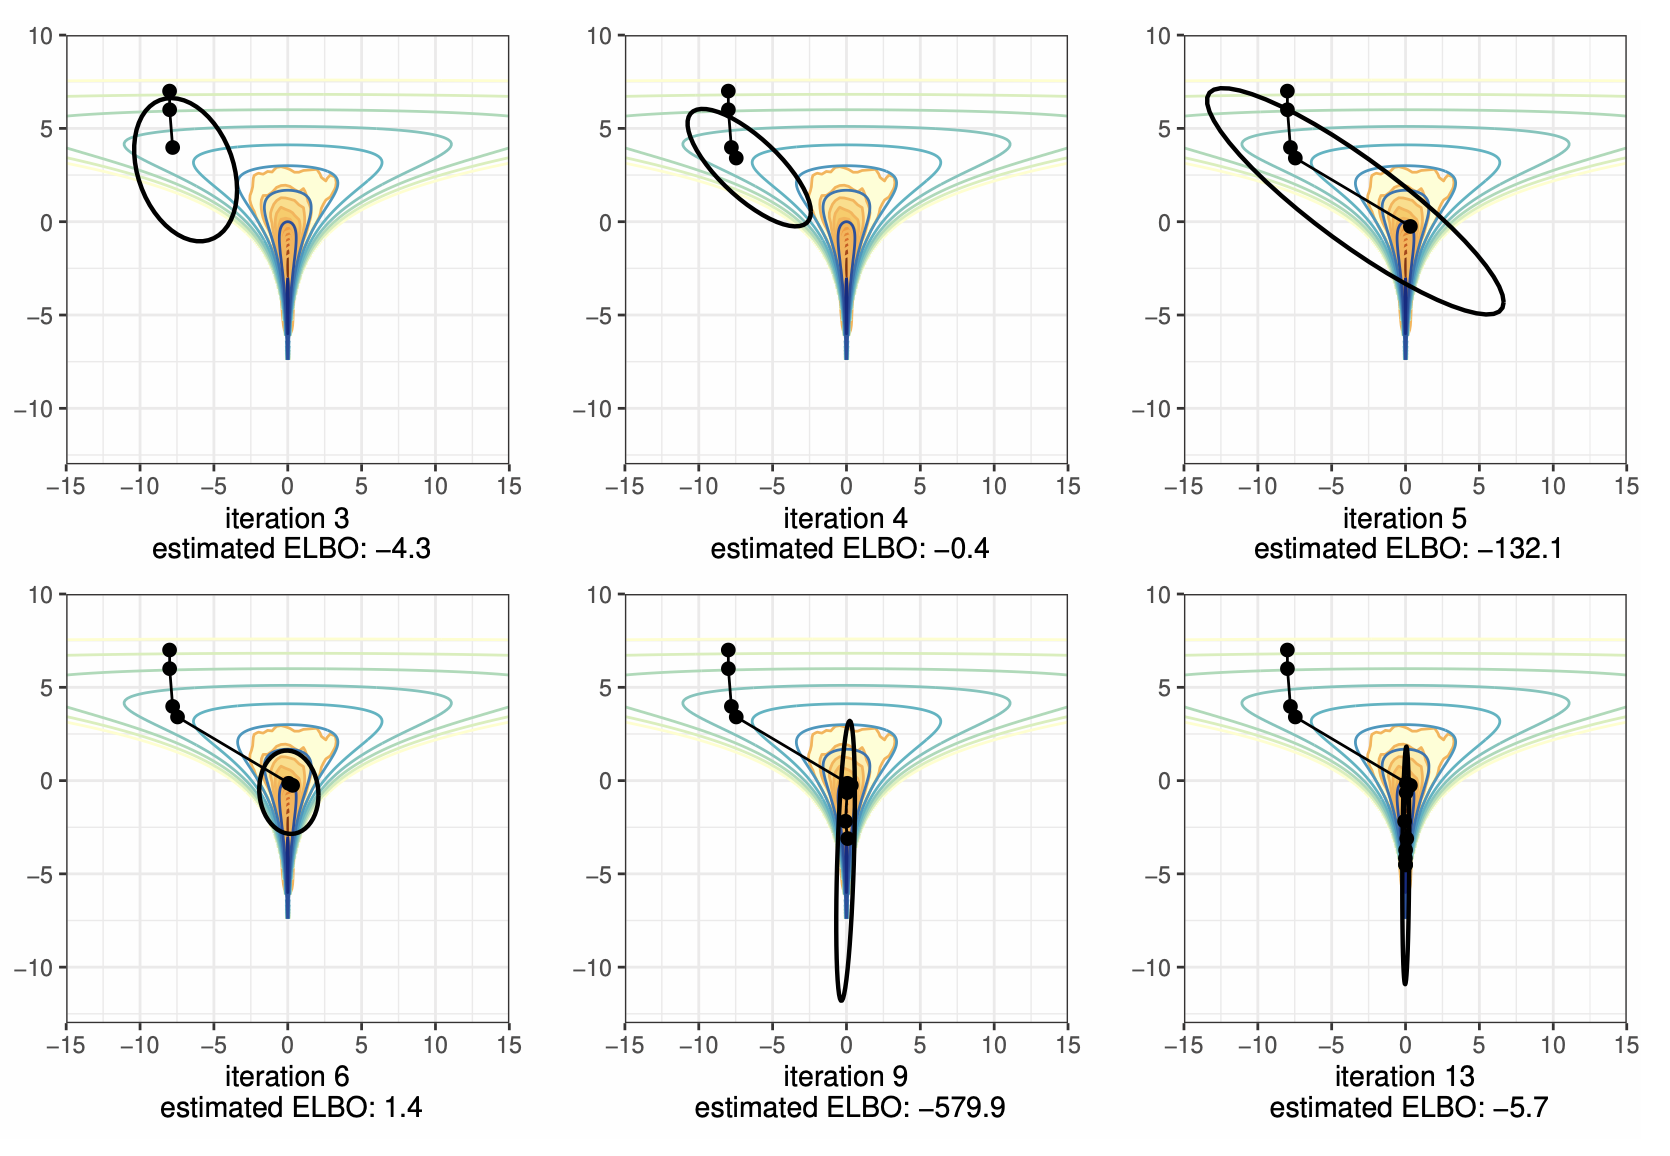
\includegraphics[width=0.65\textwidth]{img/pathfinder.png}
\end{center}

\sld{The future: normalizing flows \hfill \normalsize(Domke and Agrawal)}
\begin{itemize}
\item Like ADVI with \myemph{normalizing flows} as approximating family
  \begin{subitemize}
  \item Generate \myemph{inital} $X \sim q_X(x)$ (cf. Domke and Agrawal)
  \item \myemph{Transform} with \myemph{deep neural net}
    $f_\beta:\reals^D \rightarrow \reals^D$, $\Theta = f_\beta(X),$
    $$q_\Theta(\theta \mid \beta) = q_X\!\left(f^{-1}_\beta(\theta)\right)
    \cdot \left| \, J_{f^{-1}_\beta}(\theta) \, \right|
$$
  \item \myemph{Optimize} as in ADVI: $\beta^* =
    \textrm{arg min}_\beta \ \textrm{KL}\!\left[ \, q_\Theta(\theta \mid \beta)
    \,\big|\big|\, p(\theta \mid y) \, \right]$
\end{subitemize}
\item For VI, neural net must have \myemph{efficient Jacobian and sampling}
\item Real non-volume preserving (\myemph{RealNVP}) flows work with \myemph{JAX}
  \begin{subitemize}
  \item complementary affine layers, $\textrm{tanh}()$ non-linearity ($\approx$
    10 deep,
    12 wide)
  \item fits centered hieararchical IRT-2PL (additive + multiplicative
    + funnel)
  \end{subitemize}
\end{itemize}


\end{document}
